
\chapter{Results}

As discussed in chapter~\ref{sec:SSVEP_BCI}, the \gls{BCI} written as a practical part of this thesis has many parameters that can be changed and finding the best combination of different parameters needs thorough testing. Unfortunately, thorough testing did not fit into the scope of this thesis. The testing was performed on only one subject. By using trial and error method, settings that are shown in appendix~\ref{sec:parameters} were fixed for further testing.

After fixing the signal pipeline parameters as shown in table~\ref{tab:pipelines}, different target identification parameters were tested. This testing was performed in trials, each trial lasted 60 seconds. Four targets were used with frequencies of 5.45, 6.0, 6.67 and 7.5 Hz. The rest of the target parameters can be seen in table~\ref{tab:targets}. The application chose randomly a target that the subject had to look at and after this randomly chosen target was detected from the \gls{EEG} recording, the application chose randomly another \gls{target} that the subject had to look at and so on. New random \gls{target} was chosen only if the previous had been detected. This continued until 60 seconds had passed. If a detected \gls{target} was not the \gls{target} that the application randomly chose, then the result was classified as false positive. If a detected \gls{target} was the same as the \gls{target} that application randomly chose, then the result was classified as true positive. Accuracy was calculated by dividing the number of true positives with the total number of results.

The application gave the subject visual feedback about which \gls{target} had been detected from the \gls{EEG} recording and showed the current \gls{target} that the subject has to look at as shown in figure~\ref{fig:test_targets}. Laptop computer with \SI{60}{Hz} \gls{refresh rate} 14.0" diagonal LED-backlit HD 16:9 widescreen (1366 x 768) LCD monitor was used for displaying the \glspl{target}. For recording the brain activity, Emotiv EPOC \gls{EEG} device was used.

\begin{figure}[h]
	\centering
	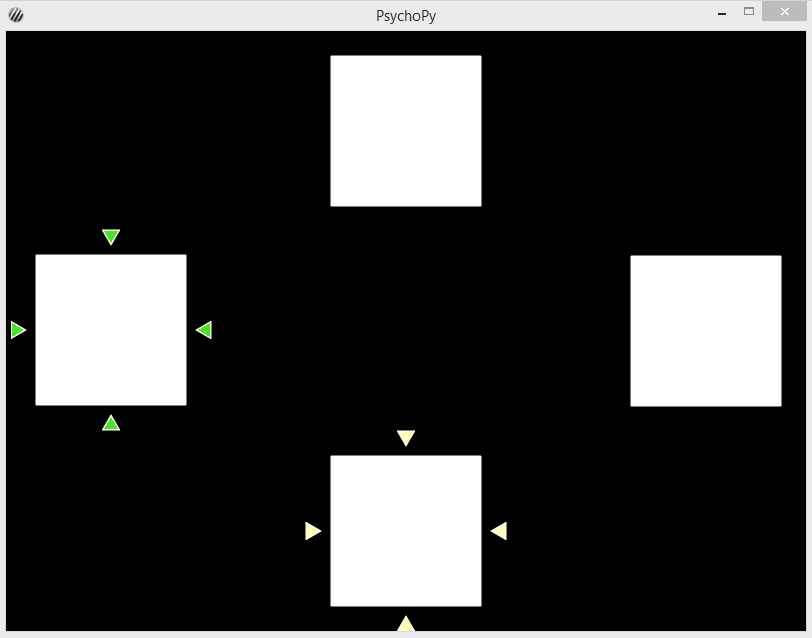
\includegraphics[width=0.6\textwidth]{test_targets.png}
	\caption{The targets used for testing the application and visual feedback for the subject. White triangles show the current target that the subject has to look and the green triangles show the target that was detected.}
	\label{fig:test_targets}
\end{figure}

The \gls{feature extraction} method's weight parameters were fixed as shown in table~\ref{tab:weights}. The method ID corresponds to the method ID in table~\ref{tab:pipelines}. Finally, different \gls{target} identification methods were tested and the results can be seen in figure~\ref{tab:results}. The \gls{target} detection time was calculated by dividing 60 seconds with the number of results in the given trial. The \gls{ITR} was calculated as shown in equation~\ref{eq:itr}.

	\begin{table}[h]
		\centering
		\begin{tabular}{|l|l|l|l|}\hline
Method	& Sensor 	& Harmonic		& Weight\\
ID		& 		 	&  				& 		\\\hline
1		& Sum of all& 1				& 6		\\\cline{2-4}
		& Sum of all& Sum of all	& 6		\\\hline
2		& All	 	& All			& 12	\\\hline
3		& O1	 	& 1				& 1		\\\cline{2-4}
		& O2	 	& 1				& 1		\\\cline{2-4}
		& O1	 	& Sum of all	& 1		\\\cline{2-4}
		& O2	 	& Sum of all	& 1		\\\cline{2-4}
		& Sum of all& Sum of all	& 1		\\\cline{2-4}
		& Sum of all& Sum of all	& 1		\\\hline
4		& All		& All			& 6		\\\hline
		\end{tabular}
		\caption{Weights of the feature extraction methods.}
		\label{tab:weights}
	\end{table}

The threshold, $k$, $m$ and $n$ in table~\ref{tab:results} are the \gls{target} identification parameters that were discussed in section~\ref{sec:identification}.

\begin{table}[h]
	\centering
	\begin{tabular}{|c|c|c|c|c|c|c|c|}\hline
Trial ID	& Target detection 	& Accuracy	& ITR (bits/min)	& Threshold&$k$ & $m$& $n$\\
			& time (sec)		& (\%)		&					&   &  &  & \\\hline
1			& 3.00				& 95.00		& 32.69				& 65& 3& 4& 3\\\hline
2			& 2.86				& 90.48		& 29.30				& 70& 3& 3& 2\\\hline
3			& 2.86				& 80.95		& 20.91				& 65& 3& 5& 3\\\hline
4			& 2.86				& 80.95		& 20.91				& 65& 3& 7& 5\\\hline
5			& 2.73				& 95.45 	& 36.55				& 65& 3& 5& 4\\\hline
6			& 2.73				& 90.91		& 31.16				& 65& 3& 4& 3\\\hline
7			& 2.73				& 90.91		& 31.16				& 65& 3& 6& 4\\\hline
8 			& 2.73	 			& 81.82 	& 22.61 			& 65& 3& 8& 5\\\hline
9 			& 2.40 				& 88.00 	& 32.01 			& 65& 3& 7& 4\\\hline
10 			& 2.40 				& 80.00 	& 24.03 			& 65& 3& 8& 4\\\hline
11 			& 2.31				& 84.62 	& 29.56 			& 65& 3& 3& 2\\\hline
12 			& 2.22 				& 81.48 	& 27.41 			& 60& 3& 4& 3\\\hline
13 			& 2.14 				& 75.00		& 22.19 			& 65& 3& 4& 2\\\hline
Average:	& $2.61\pm 0.28$ 	& $85.81\pm 6.39$	& $27.73\pm 5.11$\\\cline{1-4}
	\end{tabular}
	\caption{Results of 13 trials of testing the application. Threshold is the value that the sum of the weights of the $k$ previous results has to exceed for the corresponding target to be added to the list of results. From the list of results, a target is chosen if there are at least $n$ occurrences of the targets. The list of results has the length of $m$.}
	\label{tab:results}
\end{table}

The results presented in this section can be compared to other \glspl{BCI} that also use Emotiv EPOC headset. The results of the previous \glspl{BCI} can be seen in table~\ref{tab:emotiv_BCIs}.
